\section{SARSA}
\begin{frame}{}
    \LARGE Reinforcement Learning: \textbf{SARSA}
\end{frame}

\begin{frame}{SARSA: Overview}
    \begin{itemize}
        \item \textbf{SARSA} stands for:
        \begin{align*}
            &\text{State} \\
            \rightarrow\ &\text{Action} \\
            \rightarrow\ &\text{Reward} \\
            \rightarrow\ &\text{State}' \\
            \rightarrow\ &\text{Action}'
        \end{align*}
        \item \textbf{On-policy learning:} Learns Q-values by following the current behavior policy.
        \item \textbf{Update Rule:}
        \begin{equation*}
            Q(s, a) \leftarrow Q(s, a) + \alpha \left[ r + \gamma Q(s', a') - Q(s, a) \right]
        \end{equation*}
    \end{itemize}
\end{frame}

\begin{frame}{SARSA: Key Points}
    \begin{itemize}
        \item Uses the action the agent actually takes, not just the best possible one.
        \item Learns from the agent's real experience, not hypothetical alternatives.
        \item Tends to be safer—useful in situations where mistakes are costly.
        \item Helps the agent improve its actual behavior step by step.
    \end{itemize}
\end{frame}

\begin{frame}{SARSA vs. Q-Learning}
    \begin{itemize}
        \item The SARSA algorithm is a slight variation of the Q-Learning algorithm.
        \item Q-Learning is an \textbf{off-policy} method and uses a greedy approach to learn the Q-values.
        \item SARSA, on the other hand, is an \textbf{on-policy} method and uses the action performed by the current policy to update the Q-values.
    \end{itemize}
    \pause
    \begin{equation*}
        \textbf{Q-Learning:}\quad Q(s_t,a_t) \leftarrow Q(s_t,a_t) + \alpha \left[ r(s_t,a_t) + \gamma \max_{a'} Q(s_{t+1},a') - Q(s_t,a_t) \right]
    \end{equation*}
    \pause
    \begin{equation*}
        \textbf{SARSA:}\quad Q(s_t,a_t) \leftarrow Q(s_t,a_t) + \alpha \left[ r(s_t,a_t) + \gamma Q(s_{t+1},a_{t+1}) - Q(s_t,a_t) \right]
    \end{equation*}
\end{frame}

\begin{frame}{SARSA}
    \begin{itemize}
        \item The update equation for SARSA depends on the current state, current action, reward obtained, next state, and next action.
        \item This observation led to the naming of the learning technique as \textbf{SARSA}, which stands for \textbf{State-Action-Reward-State-Action}, symbolizing the tuple $(s, a, r, s', a')$.
        \pause
        \item Similar to DQN, there is also a Deep SARSA variant.
    \end{itemize}
\end{frame}

\begin{frame}{SARSA Algorithm}
    \begin{figure}
        \centering
        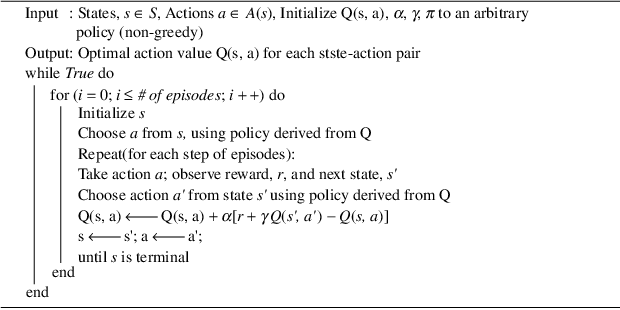
\includegraphics[width=0.9\textwidth,height=0.9\textheight,keepaspectratio]{images/dqn+sarsa/sarsa.png}
    \end{figure}

    \footnotetext{Lockery \& Peters, \href{https://www.researchgate.net/publication/228410947_Adaptive_learning_by_a_target-tracking_system}{Adaptive learning by a target-tracking system}}
\end{frame}

\begin{frame}{Q-Learning vs SARSA: Comparison Table}
    \begin{table}[h!]
        \centering
        \renewcommand{\arraystretch}{2.5}
        \begin{tabular}{lcc}
            \hline
            \textbf{Feature} & \textbf{Q-Learning} & \textbf{SARSA} \\
            \hline
            Policy Type & Off-policy & On-policy \\
            Target & $\max Q(s', a')$ & $Q(s', a')$ actually taken \\
            Exploration Aware & No & Yes \\
            Risk Sensitivity & More aggressive & More conservative \\
            Use Case & Goal-seeking behavior & Risk-aware behavior \\
            \hline
        \end{tabular}
    \end{table}
\end{frame}